\section{EDO's de 2\textordfeminine ordem lineares }




\begin{frame}
\frametitle{ EDO's de 2\fm ordem lineares}

As \dt{EDO's de 2\fm ordem linear } são equações que podem ser escritas na forma
\[y''+{\color{blue}p(t)}y'+{\color{blue}q(t)}y={\color{red}f(t)}.\]

Uma EDO de 2\fm ordem linear é dita \dt{homogênea} se ela pode ser escrita como
\begin{equation}\label{eq_hom_2}
y''+{\color{blue}p(t)}y'+{\color{blue}q(t)}y=0.
\end{equation}

\begin{exe}
\begin{enumerate}
\item EDO Linear de 2\fm ordem não-homogênea: $y''+4y=e^t\sen t$

\item EDO Linear de 2\fm ordem homogênea: $x^2y''+xy'+(x^2-1)y=0$

\item EDO não-Linear de 2\fm ordem: $yy''+y'=0$
\end{enumerate}
\end{exe}
\end{frame}



\begin{frame}
\frametitle{ }
\begin{teo}[Teorema de Existência e Unicidade das Soluções]
Considere o PVI
\[
\begin{cases}
y''+{\color{blue}p(t)}y'+{\color{blue}q(t)}y={\color{blue}f(t)}\\
y({\color{red}t_0})= {\color{red}y_0},\  y'({\color{red}t_0})={\color{red}y_1}.
\end{cases}
\]

Se {\color{blue}$p(t)$, $q(t)$ e $f(t)$} são funções contínuas em um intervalo ${\color{red}I}$ contendo ${\color{red}t_0}$, então o PVI tem {\color{blue} uma única solução definida neste intervalo}.
\end{teo}

\begin{exe} Encontre o maior intervalo no qual a solução do PVI certamente existe.
\[\begin{cases}
(t^2-3t)y''+ty'-(t+3)y=0\\
y(1)= 2,\  y'(1)=1.
\end{cases} 
\]


\end{exe}
\end{frame}

\subsection*{EDO's Homogêneas}

\begin{frame}{EDOs Lineares Homogêneas}

\begin{block}{Princípio da Superposição de Soluções}
Para \dt{EDO's lineares homogêneas}, se $y_1(t)$ e $y_2(t)$ são soluções da equação definidas em um mesmo intervalo, então $$y(t)=c_1y_1(t)+c_2y_2(t)$$
também o é, para quaisquer constantes $c_1$ e $c_2$. 
\end{block}


\begin{exe}Mostre que $y_1(x)=x$ e $y_2(x)=x^3$ são soluções da EDO mas não são soluções do PVI.
\[\begin{cases}
 x^2y''-3xy'+3y=0\\
y(1)= 2,\  y'(1)=1.
\end{cases}
\]


\end{exe}


\end{frame}

\begin{frame}

\begin{casa}
Mostre que:

\begin{enumerate}
\item As funções  $y_1=\cos x$ e $y_2=\sen x$ são soluções da EDO
$$y''+y=0$$

\item As funções $y_1=1+\cos x$ e $y_2=1+\sen x$ são soluções da EDO
$$y''+y=1,$$
mas $y_1+y_2$ não é. 

\item As funções $y_1=x^2$ e $y_2=1$ são soluções da EDO
$$y''y-xy'=0,$$
mas $y_1+y_2$ não é.
\end{enumerate}
\end{casa}
\end{frame}


%
%
%\begin{frame}
%\frametitle{  }
%\begin{scriptsize}
%
%\uncover<1->{ No último exemplo conhecíamos duas soluções da EDO, mas não uma   solução do PVI. Será possível determinar uma solução do PVI a partir dessas duas? E uma solução geral da EDO?}
%\bigskip
%
%\uncover<2->{Seja $\mathcal{S}$ o conjunto de todas as soluções da EDO do último PVI definidas no intervalo $(0,+\infty)$. Da superposição de soluções vemos que $\mathcal{S}$ é um \dt{subespaço vetorial} do espaço vetorial das funções contínuas definida no intervalo $(0,+\infty)$.}
%\bigskip
%
%\uncover<3-> {Defina a transformação 
%$$T:  \mathcal{S} \to  \R^2,\ \  \mbox{ por } \ \  T(y)=(y(1),y'(1)).  $$ 
%Note que
%\begin{itemize}
%\item $T$ é linear ( Exercício);
%\item $T$ é um isomorfismo.
%\end{itemize}
%Portanto, $\dim\mathcal{S}=2$. Com isso, duas soluções LI da EDO formam uma base de $\mathcal{S}$. Como $T(y_1)=(1,1)$ e $T(y_2)=(1,3)$ temos que $y_1$ e $y_2$ são LI, portanto qualquer solução da EDO é da forma
%$$ y(x)=c_1y_1(x)+c_2y_2(x), \forall x\in (0,+\infty)$$
%onde $c_1,c_2\in \R$.}
%
%
%\end{scriptsize}
%\end{frame}
%
%




\begin{frame}
\frametitle{ Soluções Fundamentais }
 No último exemplo vimos que $y_1(x)=x$ e $y_2(x)=x^3$, $\forall\ x\in (0,+\infty)$ são soluções da EDO $x^2y''-3xy'+3y=0$ mas não do PVI
\[\begin{cases}
 x^2y''-3xy'+3y=0\\
y(1)= 2,\  y'(1)=1.
\end{cases}
\]

Será possível determinar uma solução do PVI a partir dessas duas? E uma solução geral da EDO?

\end{frame}
%
%
%\begin{frame}
%\frametitle{}
%\begin{scriptsize}
%
%\uncover<1->{ Com isso, uma solução geral da EDO é da forma
%\begin{equation}\label{edo1}
%y(x)=c_1x+c_2x^3, \forall x\in (0,+\infty).
%\end{equation}
%Para obtermos uma solução do PVI devemos determinar $c_1$ e $c_2$  tal que $T(y)=(2,1)$, ou seja,
%$$(2,1)=T(y)=c_1(1,1)+c_2(1,3)\Rightarrow \left\{\begin{array}{l}
%c_1+c_2=2\\
%c_1+3c_2=1.
%\end{array}\right.\Rightarrow c_1=\frac{5}{2} \mbox{ e } c_2=-\frac{1}{2}.$$
%Logo, a solução do PVI é 
%$$y(x)=\frac{5x}{2}-\frac{x^3}{2}, \forall x\in (0,+\infty).$$  }
%
%
%\end{scriptsize}
%\end{frame}


%\begin{frame}
%\frametitle{ Soluções Fundamentais}
%\begin{scriptsize}
%
%
%
%\uncover<1->{Considere o PVI
%$$\left\{\begin{array}{l}
%y''+p(t)y'+q(t)y=0\\
%y(t_0)= a,\  y'(t_0)=b.
%\end{array} \right.$$
%Se $p(t)$ e $q(t)$ são contínuas, então o procedimento do exemplo anterior pode ser aplicado.}
%\bigskip
%
%\uncover<2->{Sejam $y_1$ e $y_2$ duas soluções quaisquer da EDO. Dado $\tilde{y}\in I$ qualquer, como $T_{\tilde{t}}$ é um isomorfismo, sabemos que $y_1$ e $y_2$ são LI se, e somente se, $T_{\tilde{t}}(y_1)=(y_1(\tilde{t}),y'_1(\tilde{t}))$ e $T_{\tilde{t}}(y_2)=(y_2(\tilde{t}),y'_2(\tilde{t}))$ são LI, ou ainda, se, e somente se, 
%$$\det\left(\begin{array}{cc}
%y_1(\tilde{t}) & y'_1(\tilde{t})\\
%y_2(\tilde{t}) & y'_2(\tilde{t})
%\end{array}\right)\neq 0$$}
%
%\end{scriptsize}
%\end{frame}
%
%
%\begin{frame}
%\frametitle{ }
%\begin{scriptsize}
%
%\uncover<1->{Se $y_1$ e $y_2$ são duas soluções LI, então a solução do PVI é da forma
%$y=c_1y_1+c_2y_2$. Das condições iniciais temos que
%$$
%\left\{\begin{array}{l}
% c_1y_1(t_0)+c_2y_2(t_0)=a\\
% c_1y'_1(t_0)+c_2y'_2(t_0)=b
%\end{array}\right.
%$$}
%
%\uncover<1->{Como $y_1$ e $y_2$ são  duas soluções LI, então  
%$$\det\left(\begin{array}{cc}
%y_1(t_0) & y_2(t_0)\\
%y'_1(t_0) & y'_2(t_0)
%\end{array}\right)\neq 0,$$
%Portanto o sistema linear possui única solução! }
%\bigskip
%
%\uncover<2->{ O último determinante é dito \dt{wronskiano} das funções $y_1$ e $y_2$ em $t_0$ e é denotado por $W[y_1,y_2](t_0)$. Se $y_1$ e $y_2$ são tais que $W[y_1,y_2](t)\neq 0$ para algum $t\in I$ dizemos que elas são  \dt{soluções fundamentais}.}
%
%
%\end{scriptsize}
%\end{frame}




\begin{frame}
\frametitle{Wronskiano}
Considere o PVI
\[
\begin{cases}
y''+{\color{blue}p(t)}y'+{\color{blue}q(t)}y=0\\
y({\color{red}t_0})= {\color{red}y_0},\  y'({\color{red}t_0})={\color{red}y_1}.
\end{cases}
\]
Se ${\color{blue}p(t)}$ e ${\color{blue}q(t)}$ são contínuas, então o procedimento do exemplo anterior pode ser aplicado. Dados {\color{cyan} $y_1$} e {\color{cyan} $y_2$} duas da EDO, então o PVI terá solução desde que 
\[W[{\color{cyan} y_1},{\color{cyan} y_2}]({\color{red}t_0})=
\det\left( \begin{array}{cc}
 {\color{cyan} y_1}({\color{red}t_0}) & {\color{cyan} y_2}({\color{red}t_0})  \\
{\color{cyan} y_1^\prime}({\color{red}t_0}) & {\color{cyan} y_2^\prime}({\color{red}t_0})
\end{array}
\right).\]
$W[{\color{cyan} y_1},{\color{cyan} y_2}]({\color{red}t_0})$ é chamado de {\color{blue} Wronskiano}. 


\end{frame}



\begin{frame}
\begin{teo}
Se {\color{cyan} $y_1$} e {\color{cyan} $y_2$} são soluções da EDO 
\[y''+{\color{blue}p(t)}y'+{\color{blue}q(t)}y=0,\]
e se existe ${\color{red}t_0}$ tais que $W[{\color{cyan} y_1},{\color{cyan} y_2}]({\color{red}t_0})\neq 0$, então a família de funções
\[y=c_1{\color{cyan} y_1}+c_2{\color{cyan} y_2},\]
incluem todas as soluções da EDO, chamada \dt{solução geral} da EDO. Neste caso, {\color{cyan} $y_1$} e {\color{cyan} $y_2$} são ditas \dt{soluções fundamentais}.
\end{teo}

\begin{exe}
Mostre que $y_1=t^{1/2}$ e $y_2=t^{-1}$ são soluções fundamentais da EDO
\[2t^2y''+3ty'-y=0,\ t>0\]
e determine a solução geral.
\end{exe}
\end{frame}



%
%
%
%%
%%
%\begin{frame}{Vibrações Mecânicas}
%\begin{tikzpicture}[black!75]
%		
%		% Supporting structure
%		\fill [pattern = north west lines] (-1.5,0) rectangle ++(3,.2);
%		\draw[thick] (-1.5,0) -- ++(3,0);
%		
%		% Spring + Arrows
%		\draw[] (0,0) -- ++(0,-0.25);
%		\draw[decoration={aspect=0.3, segment length=1.2mm, amplitude=2mm,coil},decorate] (0,-0.25) -- ++(0,-2.25) node[midway,right=0.25cm,black]{{\color{red}$k$}}; 
%		\draw[] (0,-2.5) -- ++(0,-0.3) node[coordinate](c1){};
%		
%		\begin{scope}[xshift=4cm]
%			% Supporting structure
%			\fill [pattern = north west lines] (-1.5,0) rectangle ++(3,.2);
%			\draw[thick] (-1.5,0) -- ++(3,0);
%			
%			% Spring + Arrows
%			\draw[] (0,0) -- ++(0,-0.25);
%			\draw[decoration={aspect=0.3, segment length=1.4mm, amplitude=2mm,coil},decorate] (0,-0.25) -- ++(0,-2.75) node[midway,right=0.25cm,black]{{\color{red}$k$}}; 
%			\draw[] (0,-3) -- ++(0,-0.3)node[coordinate](c2){} node[draw,fill=blue!70,minimum width=1cm,minimum height=0.5cm,anchor=north,label=east:{\color{blue}$m$}](M){};
%		\end{scope}
%		
%		\begin{scope}[xshift=8cm]
%			% Supporting structure
%			\fill [pattern = north west lines] (-1.5,0) rectangle ++(3,.2);
%			\draw[thick] (-1.5,0) -- ++(3,0);
%			
%			% Spring + Arrows
%			\draw[] (0,0) -- ++(0,-0.25);
%			\draw[decoration={aspect=0.3, segment length=1.5mm, amplitude=2mm,coil},decorate] (0,-0.25) -- ++(0,-3.5) node[midway,right=0.25cm,black]{{\color{red}$k$}}; 
%			\draw[] (0,-3.75) -- ++(0,-0.3)node[coordinate](c3){} node[draw,fill=blue!70,minimum width=1cm,minimum height=0.5cm,anchor=north,label=east:{\color{blue}$m$}](M){};
%		\end{scope}
%		
%		
%		\draw[dashed,gray] (c1) -- ++(3.75,0)coordinate(c22);
%		\draw[dashed,gray] (c2) -- ++(-1.5,0) coordinate(c12);
%		\draw[latex-latex] (c12)-- (c12|-c1)node[midway,left]{\small $L$};
%
%
%		
%		\draw[dashed,gray] (c22)++(0.5,0) -- ++(3.5,0)coordinate(c33);
%		\draw[dashed,gray] (c3) -- ++(-1.5,0) coordinate(c23);
%
%	    \draw[dashed,gray] (c2)++(.5,0) -- ++(2,0) coordinate(c122);
%		\draw[latex-latex] (c122)-- (c122|-c3)node[midway,left]{\small $y$};
%		
%		
%	\end{tikzpicture}
%
%Um sistema de massa-mola composto de um corpo de massa {\color{blue}$m$} preso a uma mola, com constante elástica {\color{red}$k$}, que está presa ao teto satisfaz a equação diferencial
%\[{\color{blue}m}y''+{\color{red}k}y =0.\]
%\end{frame}
%
%
%\begin{frame}{Pêndulo Simples}
%O movimento de um pêndulo simples de massa $m$ e comprimento $\ell$ é descrito pela função $\theta(t)$ que satisfaz a equação diferencial
%\[\theta''+\frac{g}{\ell}\sen\theta=0.\]
%
%\end{frame}



\begin{frame}{Vibrações Mecânicas Amortecidas}
\begin{tikzpicture}[black!75]
		
		% Supporting structure
		\fill [pattern = north west lines] (-1.5,0) rectangle ++(3,.2);
		\draw[thick] (-1.5,0) -- ++(3,0);
		
		% Spring + Arrows
		\draw[] (0,0) -- ++(0,-0.25);
		\draw[decoration={aspect=0.3, segment length=1.2mm, amplitude=2mm,coil},decorate] (0,-0.25) -- ++(0,-2.25) node[midway,right=0.25cm,black]{{\color{red}$k$}}; 
		\draw[] (0,-2.5) -- ++(0,-0.3) node[coordinate](c1){};
		
		\begin{scope}[xshift=4cm]
			% Supporting structure
			\fill [pattern = north west lines] (-1.5,0) rectangle ++(3,.2);
			\draw[thick] (-1.5,0) -- ++(3,0);
			
			% Spring + Arrows
			\draw[] (0,0) -- ++(0,-0.25);
			\draw[decoration={aspect=0.3, segment length=1.4mm, amplitude=2mm,coil},decorate] (0,-0.25) -- ++(0,-2.75) node[midway,right=0.25cm,black]{{\color{red}$k$}}; 
			\draw[] (0,-3) -- ++(0,-0.3)node[coordinate](c2){} node[draw,fill=blue!70,minimum width=1cm,minimum height=0.5cm,anchor=north,label=east:{\color{blue}$m$}](M){};
		\end{scope}
		
		\begin{scope}[xshift=8cm]
			% Supporting structure
			\fill [pattern = north west lines] (-1.5,0) rectangle ++(3,.2);
			\draw[thick] (-1.5,0) -- ++(3,0);
			
			% Spring + Arrows
			\draw[] (0,0) -- ++(0,-0.25);
			\draw[decoration={aspect=0.3, segment length=1.5mm, amplitude=2mm,coil},decorate] (0,-0.25) -- ++(0,-3.5) node[midway,right=0.25cm,black]{{\color{red}$k$}}; 
			\draw[] (0,-3.75) -- ++(0,-0.3)node[coordinate](c3){} node[draw,fill=blue!70,minimum width=1cm,minimum height=0.5cm,anchor=north,label=east:{\color{blue}$m$}](M){};
		\end{scope}
		
		
		\draw[dashed,gray] (c1) -- ++(3.75,0)coordinate(c22);
		\draw[dashed,gray] (c2) -- ++(-1.5,0) coordinate(c12);
		\draw[latex-latex] (c12)-- (c12|-c1)node[midway,left]{\small $L$};


		
		\draw[dashed,gray] (c22)++(0.5,0) -- ++(3.5,0)coordinate(c33);
		\draw[dashed,gray] (c3) -- ++(-1.5,0) coordinate(c23);

	    \draw[dashed,gray] (c2)++(.5,0) -- ++(2,0) coordinate(c122);
		\draw[latex-latex] (c122)-- (c122|-c3)node[midway,left]{\small $y$};
		
		
	\end{tikzpicture}

Considere um sistema de massa-mola composto de um corpo de massa {\color{blue}$m$} preso a uma mola, com constante elástica {\color{red}$k$}, que está presa ao teto. Se levarmos em conta um amortecimento viscoso proporcional à velocidade do corpo, então o sistema satisfaz a EDO
\[{\color{blue}m}y''+{\color{orange}\gamma} y'+{\color{red}k}y =0,\]
onde ${\color{orange}\gamma}>0$ é a constante de amortecimento.
\end{frame}


\begin{frame}
\frametitle{Equações homogêneas com coeficientes constantes }

Uma EDO linear de 2\fm ordem, homogênea, com coeficientes constantes é uma equação  da forma
\begin{equation}\label{coef_const}
ay''+by'+cy=0,\ a,b,c\in\R,\ a\neq 0.
\end{equation} 
 
\bigskip

Para resolver uma equação do tipo (\ref{coef_const}) vamos nos inspirar no caso de 1\fm ordem. Uma EDO linear homogêna de 1\fm com coeficientes constantes é da forma
\[ay'+by=0,\ a,b\in\R,\ a\neq 0.\]
Sabemos que as soluções para esta equação são $\dps y(t)=ce^{-bt/a}$. Neste caso é natural supor que uma solução da EDO (\ref{coef_const}) seja da forma $y(t)=e^{\lambda t}$ para alguma constante $\lambda$. Daí, substituindo em (\ref{coef_const}) temos que
\[a\lambda^2e^{\lambda t}+b\lambda e^{\lambda t}+ce^{\lambda t}=0\Leftrightarrow a\lambda^2+b\lambda+c=0.\]
A última equação é dita \dt{equação característica.}

\end{frame}


\begin{frame}{Raízes Reais Distintas}
\begin{exe}
 Determinar a solução geral da EDO: $y''+y'-2y=0$.
\end{exe}

\begin{block}{}

Se $\lambda_1$ e $\lambda_2$ são raízes distintas da equação característica, então a solução geral da EDO é:
\[y(t)=c_1e^{\lambda_1t}+c_2e^{\lambda_2t}, t\in \R.\]
\end{block}



\end{frame}

\begin{frame}{Raízes Reais Iguais}




\begin{exe}
 Determinar a solução geral da EDO: $y''+4y'+4y=0$
\end{exe}
\begin{block}{}
Se $\alpha$ é a única raiz da equação característica, então a solução geral da EDO é:
\[y(t)=c_1e^{\alpha t}+c_2te^{\alpha t}, t\in \R.\]


\end{block}

\end{frame}


%\begin{frame}
%
%\begin{exe} Determinar as soluções da equação:
%\begin{enumerate}[a]
%\item $y''+y'-2y=0$
%\item $y''+2y'+y=0$
%\item $y''-2y+2=0$
%\end{enumerate}
%\end{exe}
%\end{frame}

%\begin{frame}
%\frametitle{ }
%\begin{scriptsize}
%
%\uncover<1->{\begin{obs}
%
%\begin{enumerate}[a)]
%
%\item Se um dos coeficientes da EDO, $p(t)$ ou $q(t)$,  não é  contínuo no intervalo $I$, então o Wronskiano pode se anular e as funções serem LI! De fato, se no exemplo anterior procurarmos por soluções definidas em toda a reta, então as funções 
%$$ y_1=x^3\ \  \mbox{ e } \ \ 
%y_2=\left\{ \begin{array}{ll}
%x^3,& x\geq 0\\
%-x^3,& x<0
%\end{array}  \right.$$
%são soluções LI da EDO $y''-\frac{3}{x}y'+\frac{3}{x^2}y=0$ e $W[y_1,y_2](x)=0$ para todo $x\in \R.$ Isso ocorre pois as funções não são contínuas em nenhum intervalo contendo a origem. Entretanto, se restringirmos a intervalos que não contém a origem elas são LD, como por exemplo o intervalo $(-\infty,0)$, neste caso $y_1=-y_2$. Note ainda que $y_3=x$ também é solução da EDO linearmente independente das outras duas, portanto $\dim \mathcal{S}\geq 3$.
%
%\item Entretanto, se $W[y_1,y_2](t_0)\neq 0$ para algum $t_0\in I$, então $y_1$ e $y_2$ são LI em $I$. De fato, se $W[y_1,y_2](t_0)\neq 0$, então $T_{t_0}(y_1)$ e $T_{t_0}(y_2)$ são LI, daí,
%$$\alpha_1 y_1+\alpha_2y_2=0\Rightarrow \alpha_1 T_{t_0}(y_1)+\alpha_2T_{t_0}(y_2)=0\Rightarrow \alpha_1=\alpha_2=0.  $$
% 
%
%\end{enumerate} 
%
%\end{obs}}
%
%
%\end{scriptsize}
%\end{frame}





\begin{frame}
Vamos estudar inicialmente o caso
\[y''+{\color{red}\beta^2}y=0,\]
cujas soluções fundamentais são $y_1=e^{i{\color{red} \beta}t}$ e $y_2=e^{-i{\color{red} \beta}t}$. Mas como podemos escrevê-las na forma padrão  $a+bi$?
\medskip

Primeiramente, note que $u_1(t)=\cos( {\color{red} \beta}t)$ e $u_2(t)=\sen( {\color{red} \beta}t)$ também são soluções fundamentais da EDO. Portanto, 
\[y_1(t)=c_1\cos( {\color{red} \beta}t)+c_2\sen( {\color{red} \beta}t).\]
%Como $y_1(0)=1$ e $y_1'(0)=i{\color{red} \beta}$, daí, temos que $c_1=1$ e $c_2=i$. Logo,
%\[e^{i{\color{red}\beta}t}=\cos( {\color{red} \beta}t)+i\sen( {\color{red} \beta}t).\]
%Em particular, para $t=1$, temos que 
%\[e^{i{\color{red} \beta}}=\cos( {\color{red} \beta})+i\sen( {\color{red} \beta}).\]
\end{frame}

\begin{frame}{A exponencial complexa}
Até agora temos que
\[\begin{cases}
y_1(t)=e^{i{\color{red} \beta}t}\\
y_1(t)=c_1\cos( {\color{red} \beta}t)+c_2\sen( {\color{red} \beta}t).
\end{cases}\]
Como $y_1(0)=1$ e $y_1'(0)=i{\color{red} \beta}$, daí, temos que $c_1=1$ e $c_2=i$. Logo,
\[e^{i{\color{red} \beta}t}=\cos( {\color{red} \beta}t)+i\sen( {\color{red} \beta}t).\]
Em particular, para $t=1$, temos que 
\[e^{i{\color{red} \beta}}=\cos( {\color{red} \beta})+i\sen( {\color{red} \beta}).\]



\end{frame}


\begin{frame}
Curiosamente, quando  ${\color{red} \beta}=\pi$, obtemos {\color {red} a mais bela de todas as equações da matemática}:
\begin{block}{Equação de Euler}
\[e^{i\pi}+1=0.\]
\end{block}



De forma geral, obtemos:
\[e^{{\color{blue}\alpha}+{\color{red} \beta} i}=e^{\color{blue}\alpha} e^{{\color{red} \beta} i}=e^{\color{blue}\alpha}(\cos {\color{red} \beta} +i\sen {\color{red} \beta}),\]
conhecida como fórmula de Euler.
\end{frame}


\begin{frame}{Raízes Complexas}
\begin{exe}
Determine a solução geral da EDO : $y''-4y'+13y=0$.
\end{exe}
\begin{block}{ }
Se $\lambda_1={\color{blue}\alpha}+{\color{red} \beta} i$ e $\lambda_2={\color{blue}\alpha}-{\color{red} \beta} i$, então a solução geral da EDO é:
\[y(t)=e^{{\color{blue}\alpha} t}(c_1\cos({\color{red} \beta} t)+c_2\sen({\color{red} \beta} t)),\ t\in \R.\]
\end{block}
\end{frame}


\section{Vibrações Mecânicas Livres}

\subsection{Vibrações Livres}

\begin{frame}{Vibrações Mecânicas Livres}
Vimos que o modelo para um sistema massa-mola preso no teto em um meio viscoso é:
\[{\color{blue}m}y''+{\color{orange}\gamma} y'+{\color{red}k}y =0,\]
onde {\color{blue}$m$} é a massa, ${\color{red}k}>0$ é a constante elástica e   ${\color{orange}\gamma}>0$ é a constante de amortecimento.
\end{frame}

\begin{frame}{Vibrações livres não-amortecidas}
Quando ${\color{orange}\gamma}=0$, o sistema não tem amortecimento e podemos reescrever a equação:
\[y''+{\color{violet}\omega_0^2}y =0,\]
onde ${\color{violet}\omega_0^2}=\frac{{\color{red}k}}{{\color{blue}m}}$. Com isso a solução geral é:
\[y=A\cos({\color{violet}\omega_0}t)+B\sen({\color{violet}\omega_0}t),\ t\in \R.\]
 A solução pode ser reescrita como:
\[y=R\cos({\color{violet}\omega_0}t-\delta),\]
onde $A=R\cos\delta$, $B=R\sen \delta$. O \dt{período} do movimento é $T=\frac{2\pi}{{\color{violet}\omega_0}}$, a \dt{frequência} é $f=\frac{{\color{violet}\omega_0}}{2\pi}$, a \dt{amplitude} é $R$ e o parâmetro adimensional $\delta$ é chamado de \dt{fase}.

\end{frame}


\begin{frame}
O movimento descrito é chamado \dt{movimento harmônico}.
\begin{center}
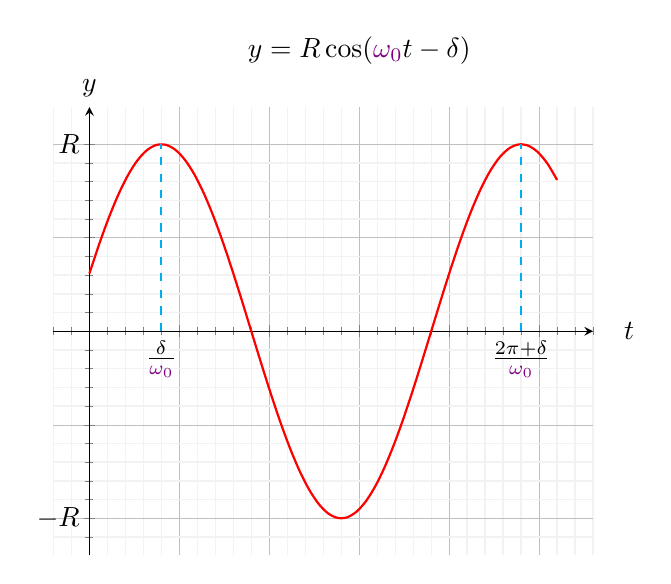
\begin{tikzpicture}
  \begin{axis}%
    [clip mode=individual,
	 grid=both,
     minor tick num=4,
     grid style={line width=.5pt, draw=gray!10},
     major grid style={line width=.2pt,draw=gray!50},
     axis lines=middle,
	 yticklabels={,,},
	 xticklabels={,,},
     enlargelimits={abs=0.2}
	]
    \addplot[domain=0:2.6,samples=50,smooth,red,thick] {cos(deg(pi*x-0.4*pi))};
\node[left ] at (0,1) {$R$};
\node[left ] at (0,-1) {$-R$};
\node[below] at (.4,0) {$\frac{\delta}{{\color{violet}\omega_0}}$};
\draw[dashed,cyan,thick] (0.4,0) -- (0.4,1);
\node[below] at (2.4,0) {$\frac{2\pi+\delta}{{\color{violet}\omega_0}}$};
\draw[dashed,cyan,thick] (2.4,0) -- (2.4,1);
\node at (3,0) {$t$};
\node at (0,1.3) {$y$};
\node at (1.5,1.5) {$y=R\cos({\color{violet}\omega_0}t-\delta)$};
  \end{axis}
\end{tikzpicture}
\end{center}

\end{frame}

\begin{frame}
\begin{center}
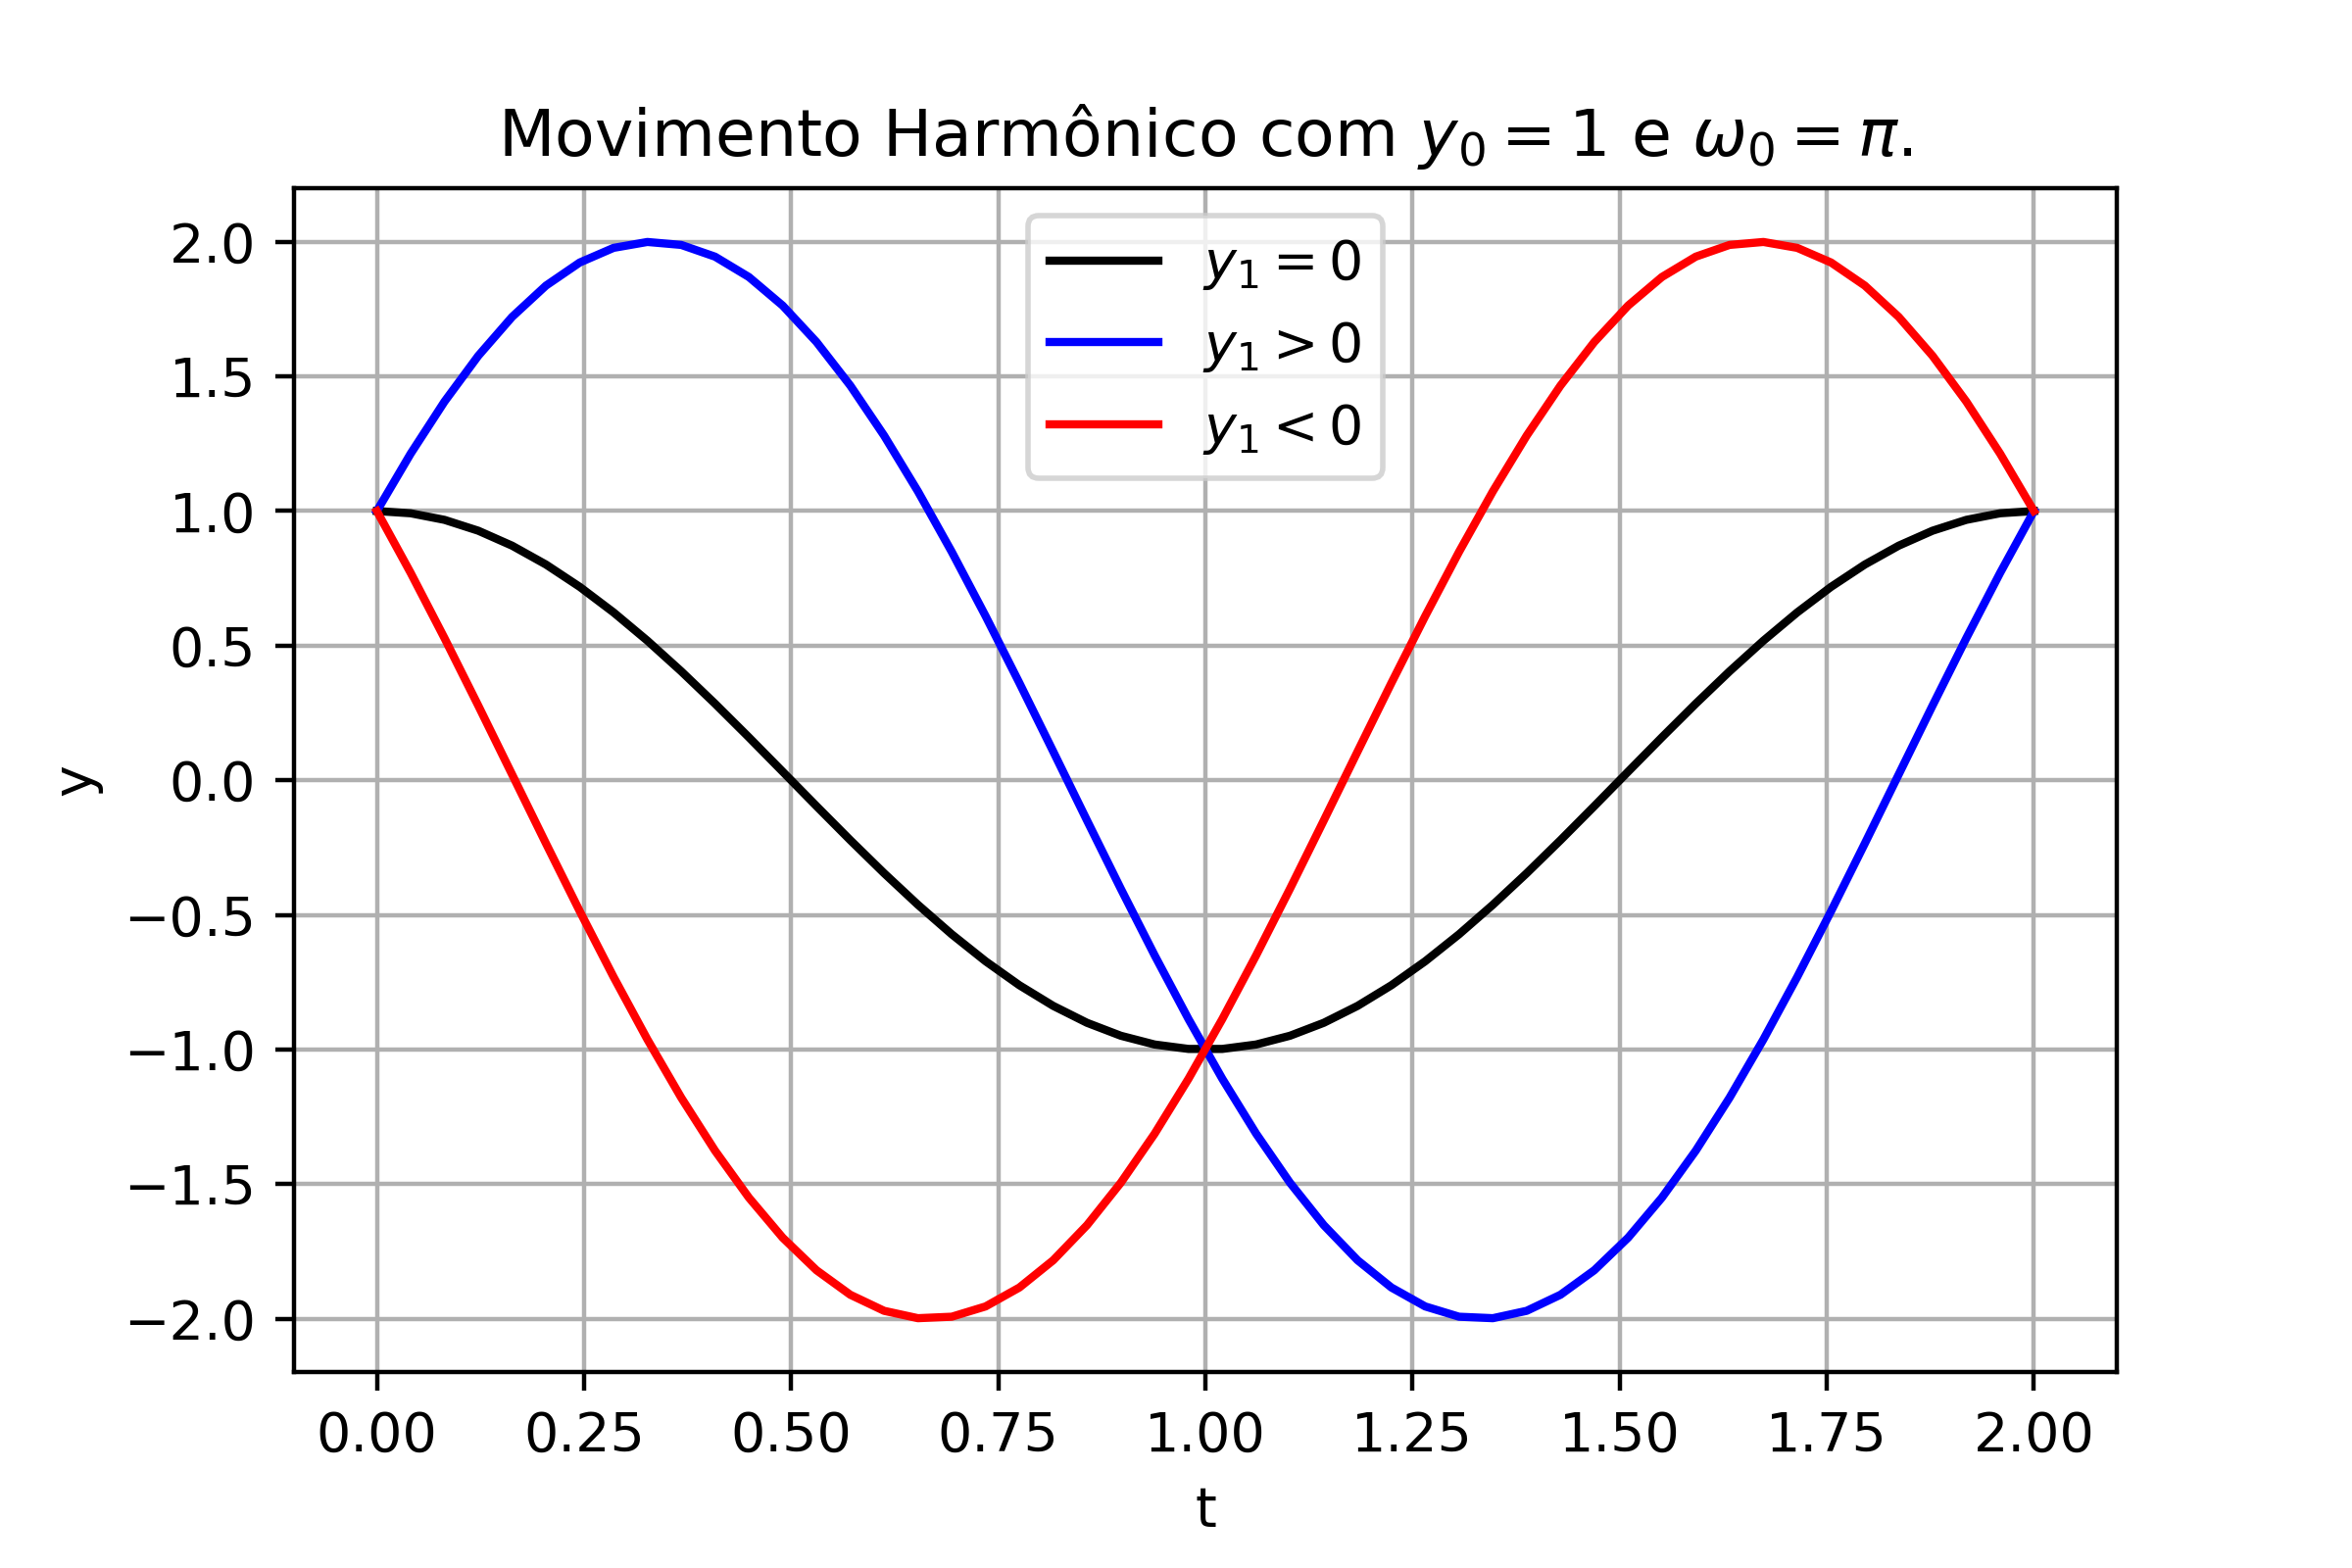
\includegraphics[scale=0.8]{osc-harm.png}
\end{center}
\end{frame}


\subsection{Vibrações Livres Amortecidas}


\begin{frame}{Vibrações Livres Amortecidas}
Quando o sistema é amortecido temos a equação:
\[{\color{blue}m}y''+{\color{orange}\gamma} y'+{\color{red}k}y =0.\]
Donde temos a equação característica:
\[{\color{blue}m}\lambda^2+{\color{orange}\gamma} \lambda+{\color{red}k} =0,\]
cujas raízes são:
\[\lambda=-\frac{{\color{orange}\gamma}}{2{\color{blue}m}}\pm \frac{\sqrt{{\color{orange}\gamma}^2-4{\color{blue}m} {\color{red}k}}}{2{\color{blue}m}},\]
o que nos fornece 3 casos:

\begin{enumerate}
\item \textbf{Superamortecimento}: \quad ${\color{orange}\gamma}^2>4{\color{blue}m} {\color{red}k}$
\item \textbf{Subamortecimento}: \qquad  ${\color{orange}\gamma}^2<4{\color{blue}m} {\color{red}k}$
\item \textbf{Amortecimento Crítico}: \ ${\color{orange}\gamma}^2=4{\color{blue}m} {\color{red}k}$
\end{enumerate}
\end{frame}


\begin{frame}{Superamortecimento}
 \[y(t)=c_1e^{\lambda_1 t}+c_2e^{\lambda_2 t},\]
onde $\lambda_1,\lambda_2<0$.

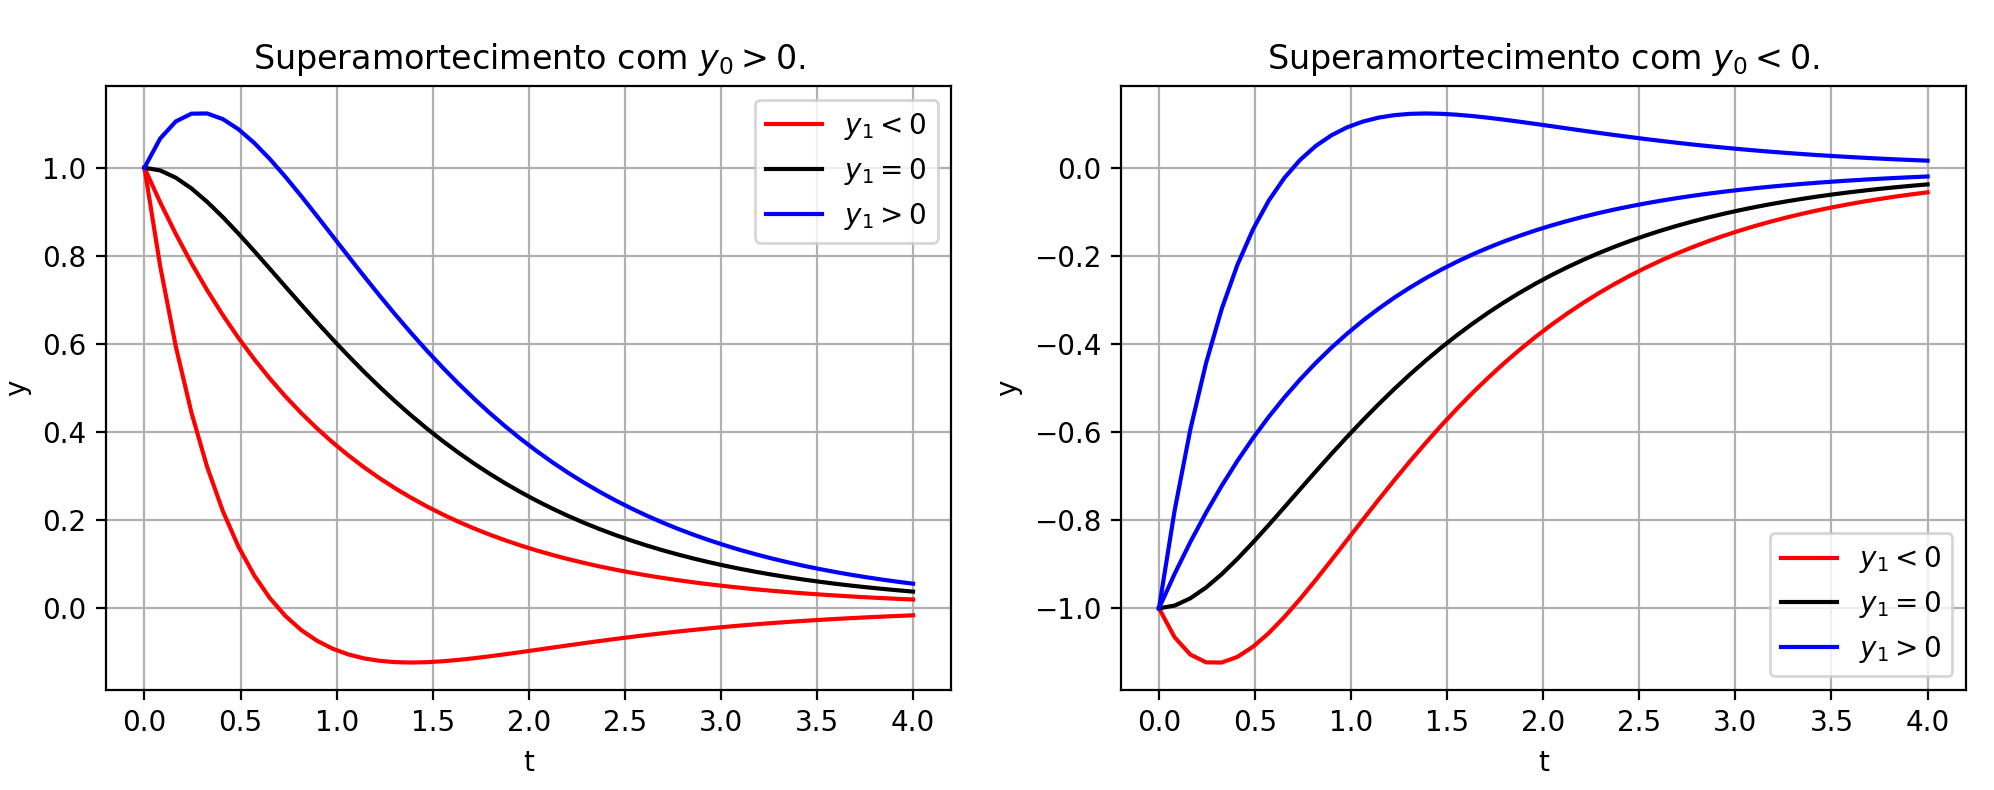
\includegraphics[scale=0.45]{osc-super.png}
%\begin{tikzpicture}
%%	\def\m{1}
%%	\def\k{2*\m}
%%	\def\g{3*\m}
%%\def\a{\g/(2*\m)}
%%\def\b{sqrt(\g*\g-4*\m*\k)/(2*\m)}
%%\def\L{-\a+\b}
%%\def\l{-\a-\b}
%  \begin{axis}%
%    [clip mode=individual,
%	 grid=both,
%     minor tick num=4,
%     grid style={line width=.5pt, draw=gray!10},
%     major grid style={line width=.2pt,draw=gray!50},
%     axis lines=middle,
%	 %yticklabels={,,},
%	 %xticklabels={,,},
%     enlargelimits={abs=0.2}
%	]
%    \addplot[domain=0:4,samples=50,smooth,red,thick] {2.7*exp(-\x)-2.1*exp(-2*\x)};
%	\addplot[domain=0:4,samples=50,smooth,cyan,thick] {0.4*exp(-\x)+0.1*exp(-2*\x)};
%	\addplot[domain=0:4,samples=50,smooth,orange,thick] {-3.3*exp(-\x)+3*exp(-2*\x)};
%%\node[left ] at (0,1) {$R$};
%%\node[left ] at (0,-1) {$-R$};
%%\node[below] at (.4,0) {$\frac{\delta}{{\color{violet}\omega_0}}$};
%%\draw[dashed,cyan,thick] (0.4,0) -- (0.4,1);
%%\node[below] at (2.4,0) {$\frac{2\pi+\delta}{{\color{violet}\omega_0}}$};
%%\draw[dashed,cyan,thick] (2.4,0) -- (2.4,1);
%%\node at (3,0) {$t$};
%%\node at (0,1.3) {$y$};
%%\node at (1.5,1.5) {$y=R\cos({\color{violet}\omega_0}t-\delta)$};
%  \end{axis}
%\end{tikzpicture}


\end{frame}


\begin{frame}{Subamortecimento}
A solução é da forma
 \[y(t)=e^{-\frac{{\color{orange}\gamma}t}{2{\color{blue}m}}}(A\cos(\mu t)+B\sen(\mu t)),\]
onde $\mu=\frac{\sqrt{4{\color{blue}m {\color{red}k}}-{\color{orange}\gamma}^2}}{2{\color{blue}m}}$.
Que pode ser reescrita como
 \[y(t)=Re^{-\frac{{\color{orange}\gamma}t}{2{\color{blue}m}}}\cos(\mu t-\delta),\]
onde $A=R\cos\delta$ e $B=R\sen\delta$.

\begin{center}
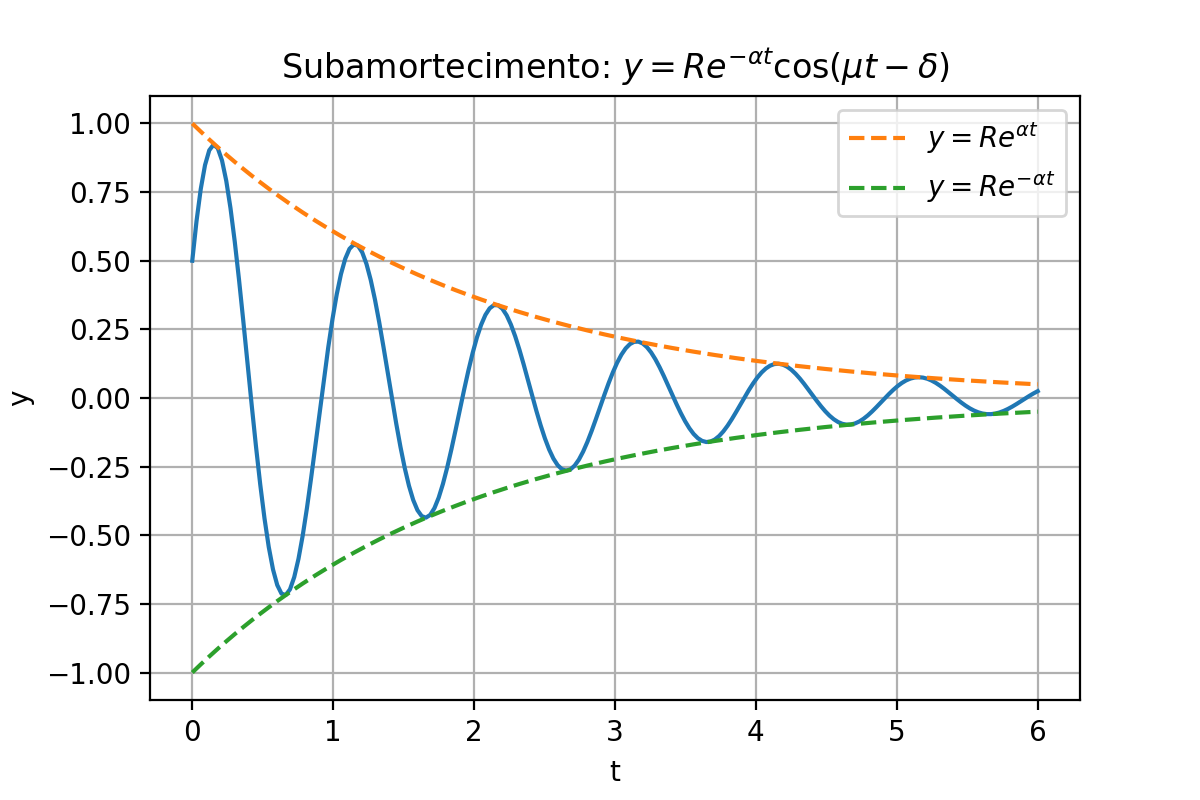
\includegraphics[scale=0.45]{osc-subarm.png}
\end{center}
\end{frame}




\begin{frame}{Amortecimento crítico}
A solução é da forma
 \[y(t)=(A+Bt)e^{-\frac{{\color{orange}\gamma}t}{2{\color{blue}m}}}.\]


\begin{center}
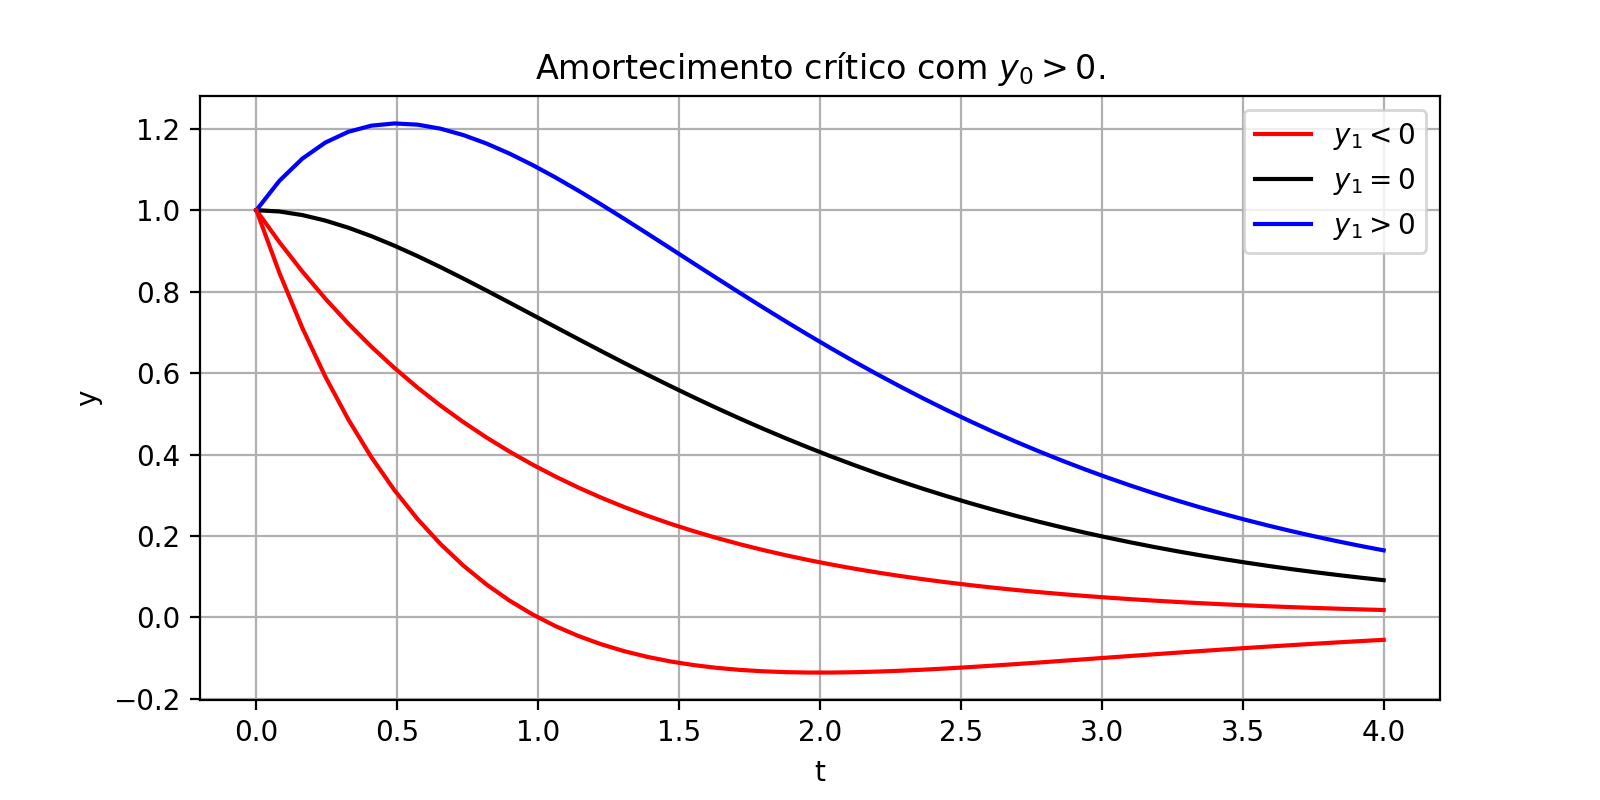
\includegraphics[scale=0.5]{osc-critico.png}
\end{center}
\end{frame}

\begin{frame}
\begin{casa}
Esboce os gráficos das soluções dos problemas abaixo.
\begin{enumerate}
\item Suponha que uma massa de 4,5 kg estica uma mola x5cm. A massa é deslocada  2,5 cm para baixo e depois colocada em movimento  com uma velocidade inicial de apontando para cima de 30 cm/s. 

\item Uma massa de 20g estica uma mola 5 cm. Suponha que a massa também está presa a um amortecedor viscoso com uma constante de amortecimento de 400 dinas$\cdot$s/cm e que a massa é puxada pra baixo mais 2 cm de depois é solta. 
\end{enumerate}
\end{casa}
\end{frame}

%
%\begin{frame}
%\frametitle{ }
%\begin{scriptsize}
%
%\uncover<1->{\begin{exe} Mostre que $y_1(t)=\cos bt$ e $y_2(t)=\sen bt$ são soluções fundamentais da equação
%$$y''+b^2y=0$$
%
%\end{exe} }
%
%Usando o exemplo anterior podemos estender a função exponencial para os números complexos. Queremos definir $y(t)=e^{zt}$ para números complexos $z=a+bi$ de forma que satisfaça as propriedades
%\begin{align*}
%& e^{(a+ib)t}=e^{at}e^{ibt}\\
%& \frac{d}{dt}(e^{zt})=ze^{zt}.
%\end{align*}
%Note que a função $w(t)=e^{ibt}$ é solução do PVI
% $$\left\{\begin{array}{l}
% y''+b^2y=0 \\
% y(0)=1,\  y'(0)=ib.
% 
%\end{array}  \right.$$
%Assim, do exemplo anterior, como $y_1(t)=\cos bt$ e $y_2(t)=\sen bt$ são soluções fundamentais da EDO, temos que
%$$z(t)=\cos bt+i\sen bt.$$
%
%
%
%\end{scriptsize}
%\end{frame}
%
%
%
%\begin{frame}
%\frametitle{ }
%\begin{scriptsize}
%
%\uncover<1->{ Portanto, das propriedades de exponencial, obtemos que
%$$e^{a+bi}=z(1)=e^a(\cos b+i\sen b),$$
%conhecida como \dt{fórmula de Euler}.}
%
%\end{scriptsize}
%\end{frame}
%
%
%\begin{frame}
%\frametitle{Equações homogêneas com coeficientes constantes }
%\begin{scriptsize}
%
%\uncover<1->{Uma EDO linear de 2\fm ordem, homogênea, com coeficientes constantes é uma equação  da forma
%\begin{equation}\label{coef_const}
%ay''+by'+cy=0,\ a,b,c\in\R,\ a\neq 0.
%\end{equation} 
% }
%\bigskip
%
%\uncover<2->{Para resolver uma equação do tipo (\ref{coef_const}) vamos nos inspirar no caso de 1\fm ordem. Uma EDO linear homogêna de 1\fm com coeficientes constantes é da forma
%$$ay'+by=0,\ a,b\in\R,\ a\neq 0.$$
%Sabemos que as soluções para esta equação são $\dps y(t)=ce^{bt/a}$. Neste caso é natural supor que uma solução da EDO (\ref{coef_const}) seja da forma $y(t)=e^{\lambda t}$ para alguma constante $\lambda$. Daí, substituindo em (\ref{coef_const}) temos que
%$$a\lambda^2e^{\lambda t}+b\lambda e^{\lambda t}+ce^{\lambda t}=0\Leftrightarrow a\lambda^2+b\lambda+c=0.$$
%A última equação é dita \dt{equação característica.}}
%
%\uncover<3->{\begin{exe} Determinar as soluções da equação:
%\begin{enumerate}[a)]
%\item $y''+y'-2y=0$
%\item $y''+2y'+y=0$
%\item $y''-2y+2=0$
%\end{enumerate}
%\end{exe}}

%
%\end{scriptsize}
%\end{frame}

\subsection*{EDO's Não-Homogêneas}



\begin{frame}
\frametitle{Equações não-homogêneas }
%\begin{scriptsize}

É fácil ver que se {\color{red}$y_p(t)$} é uma solução de uma EDO não-homogênea
\[y''+{\color{blue}p(t)}y'+{\color{blue}q(t)}y={\color{blue}f(t)},\]
 {\color{cyan}$y_1$} e {\color{cyan}$y_2$} são soluções fundamentais da EDO homogênea correspondente, então a solução geral da equação não-homogênea é
\[y(t)={\color{red}y_p(t)}+c_1{\color{cyan}y_1(t)}+c_2{\color{cyan}y_2(t)}.\]



\end{frame}

\begin{frame}
\begin{exe}
Se no modelo de vibrações mecânicas existir uma força externa $F=F(t)$, então teremos um problema de \dt{oscilação forçada} que é modelado pela  seguinte equação não-homogênea:
\[{\color{blue}m}y''+{\color{orange}\gamma} y'+{\color{red}k}y =F(t).\]

Neste caso, como determinar a solução do  seguinte problema  cuja força externa é periódica?
\[y''+2y'+y=2\cos(t).\]
\end{exe}
\end{frame}

\begin{frame}
\begin{center}
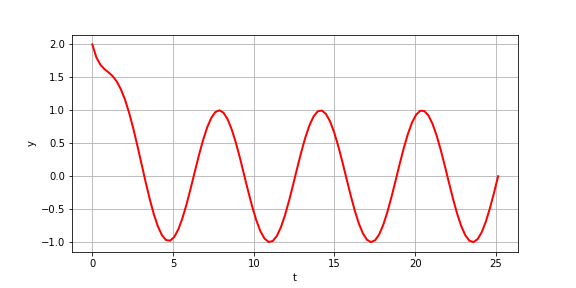
\includegraphics[scale=0.5]{osc-for-ex1.png}
\end{center}
\end{frame}




\begin{frame}
\frametitle{Método dos Coeficientes a Determinar }

\uncover<1->{Este método funciona para qualquer EDO não-homogênea com coeficientes constantes
\[ay''+by'+cy=F_1(t)+F_2(t)+\cdots+F_k(t),\]
onde  
\[F_i(t)=e^{{\color{blue}\alpha }t}[(a_0+\ldots+a_nt^{{\color{teal}n}}) \cos({\color{red}\beta}t)+(b_0+\ldots+b_mt^{{\color{teal}m}})\sen({\color{red}\beta} t)].\]

Neste caso, deve-se procurar, para cada $F_i$, uma solução particular da forma
\[y_p(t)=t^{{\color{cyan}s}}e^{{\color{blue}\alpha } t}[(A_0+\ldots+A_qt^{\color{teal}q})\cos({\color{red}\beta} t)+(B_0+\ldots+B_qt^{{\color{teal}q}})\sen({\color{red}\beta} t)],\]
em que ${\color{teal}q}=\max\{{\color{teal}n},{\color{teal}m}\}$,  ${\color{cyan}s}$ é o menor inteiro não-negativo que garante que  nenhuma parcela de $y_p$ seja solução da equação homogênea correspondente e $A_0,\ldots,A_q,B_0,\ldots,B_q$ são coeficientes a serem determinados. 



}

\end{frame}

\begin{frame}
\begin{exe} Encontre a solução geral das seguintes equações:
\begin{enumerate}[a]
\item $y''+y'=2+t^2$.
\item $y''-2y'+y=e^{t}+t$
\item $y''+4y=e^t\cos t$

\end{enumerate}
\end{exe}
\end{frame}


\begin{frame}{Vibrações Mecânicas Forçadas}
conteúdo...
\end{frame}



\begin{frame}
\frametitle{ Método da Variação dos Parâmetros}
%\begin{scriptsize}

Este método funciona para qualquer EDO linear de 2\fm ordem 
\[y''+{\color{blue}p(t)}y'+{\color{blue}q(t)}y={\color{blue}f(t)},\]
para o qual se conheça duas soluções fundamentais da equação homogênea correspondente em um intervalo $I$ onde o wronskiano é não nulo.
\bigskip

Sabemos que a solução geral da equação homogênea correspondente é
$$y(t)={\color{red}c_1}y_1(t)+{\color{red}c_2}y_2(t).$$
O método da variação dos parâmetros consiste em procurar uma solução particular da EDO não homogênea que tenha  a forma da solução geral da homogênea, mas substituindo os parâmetros $c_1$ e $c_2$ por funções a determinar $u_1(t)$ e $u_2(t)$, respectivamente, ou seja, da forma
\[y(t)={\color{red}u_1(t)}y_1(t)+{\color{red}u_2(t)}y_2(t),\]
com a condição de que
\[{\color{red}u'_1(t)}y_1(t)+{\color{red}u'_2(t)}y_2(t)=0\]

%\end{scriptsize}
\end{frame}

\begin{frame}{Fórmula Geral}
Resolvendo-se o sistema anterior, chega-se a:
\[{\color{red}u_1(t)=-\int \frac{y_2(t)f(t)}{W[y_1,y_2](t)}\,dt,\ \text{ e } u_2(t)=\int \frac{y_1(t)f(t)}{W[y_1,y_2](t)}\,dt}\]
\begin{exe}
 Encontre a solução do PVI
 $$\left\{
 \begin{array}{l}
 y''+y=\sec t\\
 \\
 y(0)=1,\ y'(0)=-2.
 \end{array}\right.$$
 \end{exe} 
\end{frame}


\begin{frame}
\frametitle{ }
\begin{exe} 

\begin{enumerate}
\item Determine a solução geral das EDO 
\[y''+2y'+2y=\frac{e^{-x}}{\cos^3(x)}.\]
\item Verifique que $y_1(t)=t^2$ e $y_2(t)=t^{-1}$ são soluções fundamentais da EDO no intervalo $(0,\infty)$
\[t^2y''-2y=3t^2-1\]
e determine a soução geral.
\end{enumerate}
\end{exe}
%\end{scriptsize}
\end{frame}



%
%
%\begin{frame}
%\frametitle{ }
%
%
%\center{\Huge{FIM !!!}
%\bigskip
%
%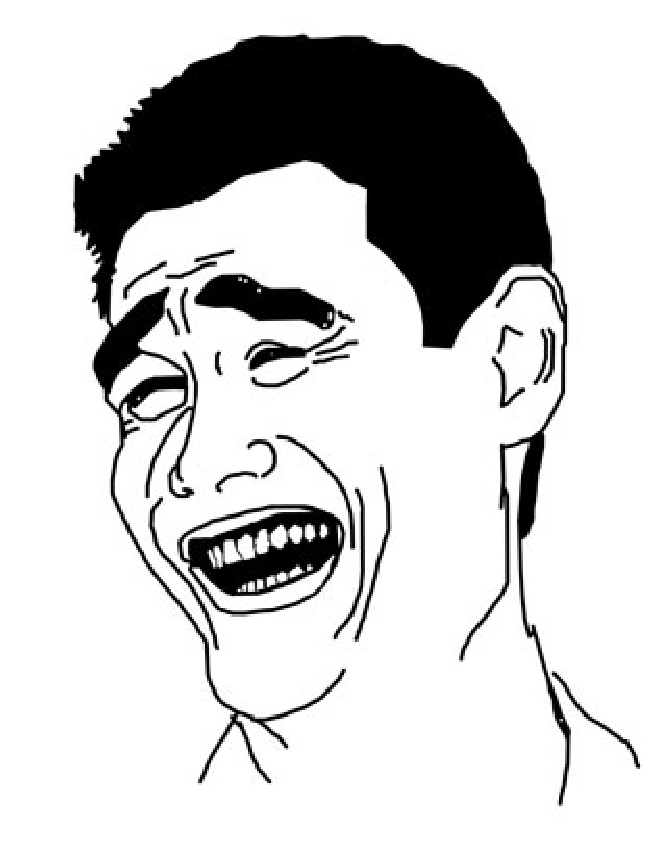
\includegraphics[scale=0.4]{ming.eps}}
%
%\end{frame}



